% =====================================================================
%  N3: one .ohq model file, every entry point.
%  Build: pdflatex fig_toolchain.tex && cp fig_toolchain.pdf figures/N3_toolchain.pdf
% =====================================================================
\documentclass[border=4pt]{standalone}
\usepackage[T1]{fontenc}
\usepackage{helvet}
\renewcommand\familydefault{\sfdefault}
\usepackage{tikz}
\usetikzlibrary{arrows.meta,positioning,calc,fit,backgrounds}

\definecolor{ohqblue}{HTML}{1F5C8B}
\definecolor{ohqteal}{HTML}{2A9D8F}
\definecolor{ohqrust}{HTML}{E76F51}
\definecolor{ohqgrey}{HTML}{6B7280}
\definecolor{bandfill}{HTML}{EDF1F4}

\begin{document}
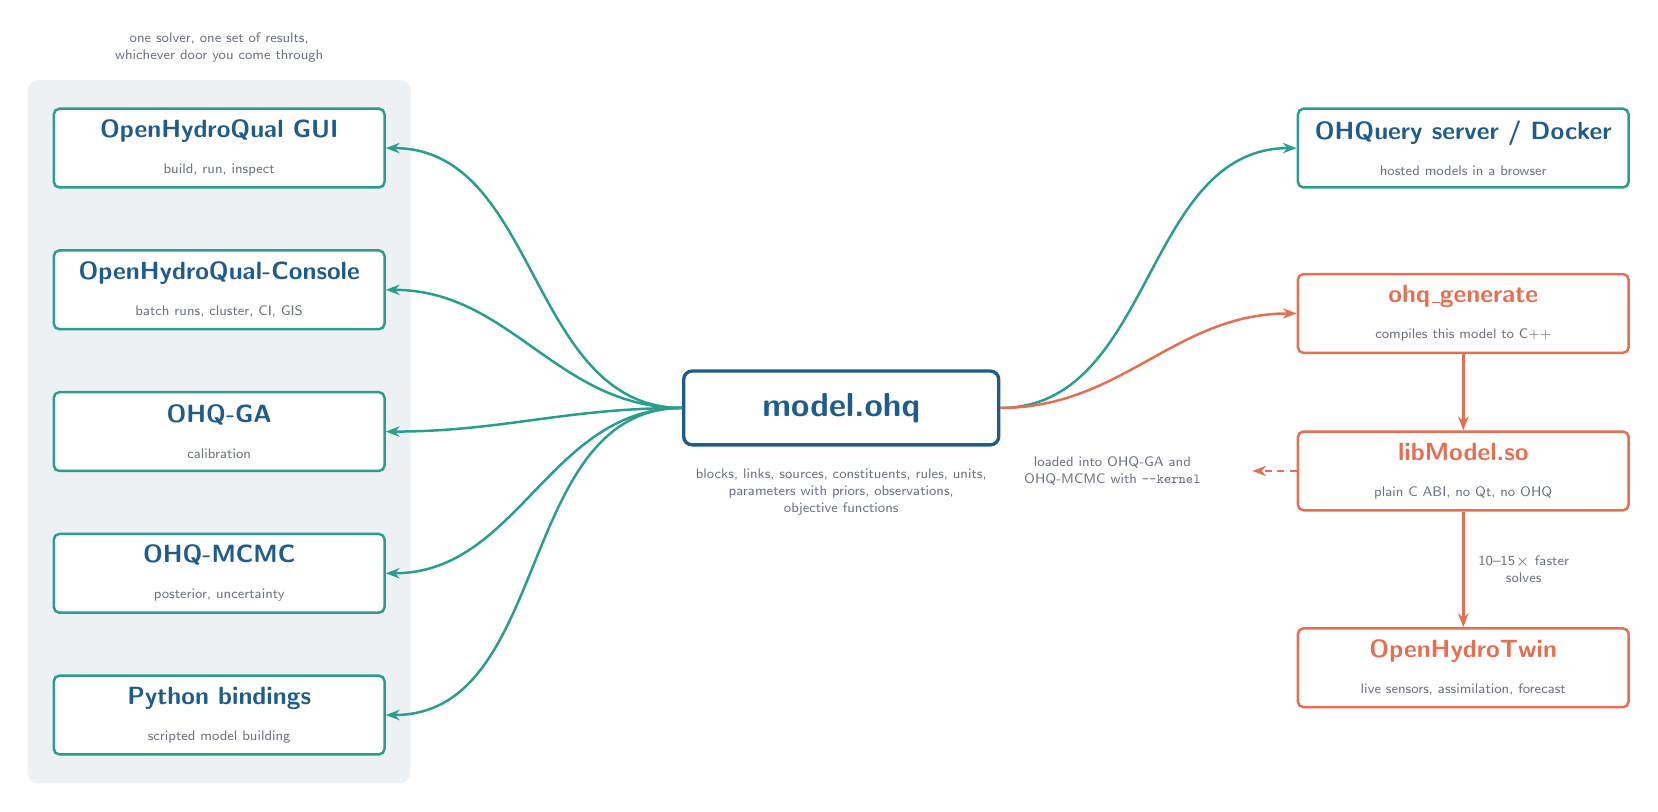
\begin{tikzpicture}[
  font=\sffamily,
  file/.style={draw=ohqblue, line width=1.2pt, fill=white, rounded corners=3pt,
               align=center, inner sep=8pt, minimum width=40mm},
  entry/.style={draw=ohqteal, line width=0.9pt, fill=white, rounded corners=2pt,
                align=center, inner sep=4pt, minimum width=42mm,
                minimum height=10mm},
  kernel/.style={draw=ohqrust, line width=0.9pt, fill=white, rounded corners=2pt,
                 align=center, inner sep=4pt, minimum width=42mm,
                 minimum height=10mm},
  arr/.style={-{Stealth[length=5pt]}, ohqteal, line width=0.9pt},
  arrr/.style={-{Stealth[length=5pt]}, ohqrust, line width=0.9pt},
  lbl/.style={font=\tiny, text=ohqgrey, inner sep=2pt, align=center},
]

\def\hdr#1{\textbf{\color{ohqblue}\small #1}}
\def\hdrr#1{\textbf{\color{ohqrust}\small #1}}
\def\sub#1{\\[1pt]\color{ohqgrey}\tiny #1}

% ---------------- the model file ------------------------------------
\node[file] (ohq) at (0,0) {\textbf{\color{ohqblue}\large model.ohq}};
\node[lbl, anchor=north, text width=52mm] at ([shift={(0,-6pt)}]ohq.south)
  {blocks, links, sources, constituents, rules, units,\\
   parameters with priors, observations,\\
   objective functions};

% ---------------- interactive and headless entry points -------------
\node[entry] (gui)  at (-7.9, 3.3) {\hdr{OpenHydroQual GUI}\sub{build, run, inspect}};
\node[entry] (cons) at (-7.9, 1.5) {\hdr{OpenHydroQual-Console}\sub{batch runs, cluster, CI, GIS}};
\node[entry] (ga)   at (-7.9,-0.3) {\hdr{OHQ-GA}\sub{calibration}};
\node[entry] (mcmc) at (-7.9,-2.1) {\hdr{OHQ-MCMC}\sub{posterior, uncertainty}};
\node[entry] (py)   at (-7.9,-3.9) {\hdr{Python bindings}\sub{scripted model building}};

\foreach \n in {gui,cons,ga,mcmc,py}
  \draw[arr] (ohq.west) to[out=180, in=0] (\n.east);

\begin{scope}[on background layer]
  \node[fill=bandfill, rounded corners=4pt, fit=(gui)(py),
        inner xsep=9pt, inner ysep=10pt] (leftband) {};
\end{scope}
\node[lbl, anchor=south, text width=46mm] at ([shift={(0,4pt)}]leftband.north)
  {one solver, one set of results,\\whichever door you come through};

% ---------------- served and compiled paths -------------------------
\node[entry]  (web)  at (7.9, 3.3) {\hdr{OHQuery server / Docker}\sub{hosted models in a browser}};
\node[kernel] (gen)  at (7.9, 1.2) {\hdrr{ohq\_generate}\sub{compiles this model to C++}};
\node[kernel] (lib)  at (7.9,-0.8) {\hdrr{libModel.so}\sub{plain C ABI, no Qt, no OHQ}};
\node[kernel] (twin) at (7.9,-3.3) {\hdrr{OpenHydroTwin}\sub{live sensors, assimilation, forecast}};

\draw[arr]  (ohq.east) to[out=0, in=180] (web.west);
\draw[arrr] (ohq.east) to[out=0, in=180] (gen.west);
\draw[arrr] (gen.south) -- (lib.north);
\draw[arrr] (lib.south) -- node[lbl, right, xshift=3pt]
  {10--15$\times$ faster\\solves} (twin.north);

% the compiled kernel is what the headless estimators load
\node[lbl, anchor=east, text width=34mm] (kn) at ([shift={(-16pt,0)}]lib.west)
  {loaded into OHQ-GA and\\OHQ-MCMC with \texttt{-{}-kernel}};
\draw[arrr, dashed, dash pattern=on 2.5pt off 2pt] (lib.west) -- (kn.east);

\end{tikzpicture}
\end{document}
